\chapter{User Study for Identifying Functions of Tweets}
\label{chap:user}

% More details on the paper.
\chapref{chap:analysis} described the analyses performed on the data and the resulting conclusion that only a small portion of indicative tweets can be recovered from the article they link to if viewed as an extractive summarization problem. This conclusion suggests that the next step should be to gain more knowledge about the relation between the tweet and the article, specifically why the user chose to write the tweet. This information would enable us to infer whether a tweet can actually be generated from summarizing the text in the article and if so, lead us to a strategy that would be the most appropriate for this task. We explore the task of collecting more information about the dataset in this chapter. We run a user study on Amazon Mechanical Turk, a crowdsourcing platform that enables researchers to put up huge samples of data along with surveys, quizzes, and simple tasks to be solved by people over the world. In this study, we asked the users whether a tweet is an advertisement or a summary of the article. We describe the process of running the user study and analysis of results obtained from the user study.

\section{Functions of Tweets}
\label{sec:funcs}
% Preliminary recommendations on text typology
One aspect of gaining more knowledge would be asking what the \textit{`function'} of the tweet is. While many possible definitions of `function' are possible, our working definition of the term, introduced in \chapref{chap:background}, is why the user chose to share the article with the particular text written in the tweet. If the function of the tweet is known, it might be possible to predict the appropriateness of extractive methods for generating tweets. For example, if the function of the tweet is to be an advertisement for a particular product and the text contains the description of the features of the product, then intuitively, the tweet would likely be an extractive summary of the text. On the other hand, if the tweet were an attention grabbing title to merely bring traffic to the text, it would be more likely to be a generalized title, than a summary of the actual text. To identify these functions, we first examined multiple previous studies aiming to classify functions of tweets, discussed in \secref{sec:related_user}. Based on these studies, we isolated the functions and finalized the questions to be asked about the tweets. The data was then given to human evaluators to annotate in a user study.


\section{User Study Design}

The following sections describe the details surrounding the design and execution of the user study. 

\subsection{Questions Used in the User Study}
\label{sec:qs}

The questions to be asked in the user study with respect to each tweet-article pair came from our definition of the function of a tweet, described in \secref{sec:funcs}. The final questions that were used are shown in \tabref{tab:mturkqs}.  

\begin{table}[!t]
\centering
\begin{tabular}{|p{0.15\linewidth}|p{0.8\linewidth}|}
\hline
\textbf{Question 1:} Advertisement & Does the tweet explicitly encourage the reader to visit the link and read the original article? \\ \hline
\textbf{Question 2:} Summary & Does the tweet contain some information from the article, or summarize the article?             \\ \hline
\end{tabular}
\caption{Questions used in user study}
\label{tab:mturkqs}
\end{table} 

The type of articles being referenced, and the possible reasons these might be shared gave the list of possible functions. Using these and earlier studies, we suggest a list of relevant functions of tweets for our data: promote a product or an article or convey information from the article. These functions will ideally help provide parameters for generating tweets. The idea behind these functions will be discussed in the following paragraphs. 

\paragraph{Advertisement question} If the tweet references a newspaper article, it might be promoting the article, in the sense of attracting people to read the article in detail. This kind of tweet would try to sensationalize the material. It could either tweet the headline of the article directly, or summarize the headline itself further, or simply say something to the effect of `Check this out' or `This is worth a read' and then further tag the article with the use of appropriate hashtags indicating the contents of the text.

Example: ``Check out this article! \{url\}" or ``Look what this says! \{url\}"

\paragraph{Summary question} Secondly, the tweet could single out a particular piece of information or opinion directly from the article, either to agree with it or to express the importance of the sentence or phrase in the article according to the author of the tweet. It could also be a short summary of the text of the article either with the aim of inviting readers or just to inform readers about the contents of the article.

Example: ``Winter approaching, ways to stay safe from flu season: \{url\}"

These questions were presented separately in two different studies. We found a possibility that workers were viewing the questions in the pilot studies as either/or questions, where the answer to only one of them could be `yes'. Thus, separating the questions guaranteed an unbiased opinion about each question without any assumptions.

A third possible question of whether the tweet expressed an emotion towards the article, and if so, whether it was a positive or negative emotion was also considered. However, it was not included in the final study, and will be discussed in \secref{sec:pilot}

% \section{Running User Study on Amazon Mechanical Turk}

% Amazon Mechanical Turk is a crowdsourcing platform that enables researchers to put up huge samples of data along with surveys, quizzes, and simple tasks to be solved by people over the world.

%  \paragraph{Questions used} We devised three questions based on the possible functions described above, and different phrasing for these was experimented with. Each question asked if the tweet served that particular function with respect to the article. The question about whether the tweet conveyed any emotion about the article was dropped going forward with the rest of the studies because of the difficulty in distinguishing the difference between emotion towards the article vs emotion expressed in the article itself.


\subsection{Running the User Study}

\figref{fig:q1} and \figref{fig:q2} show an example of what a HIT (task on Mechanical Turk) for the two questions looked like to the user, respectively. For each of the questions, the first part of the figure shows the instructions involved as well as examples for every possible answer to the question asked. The tweet, the title that was extracted and the entire text of the article was then presented to help the workers make a decision about their answer.  

\begin{figure}[!htbp]
  \centering 
  \subfloat{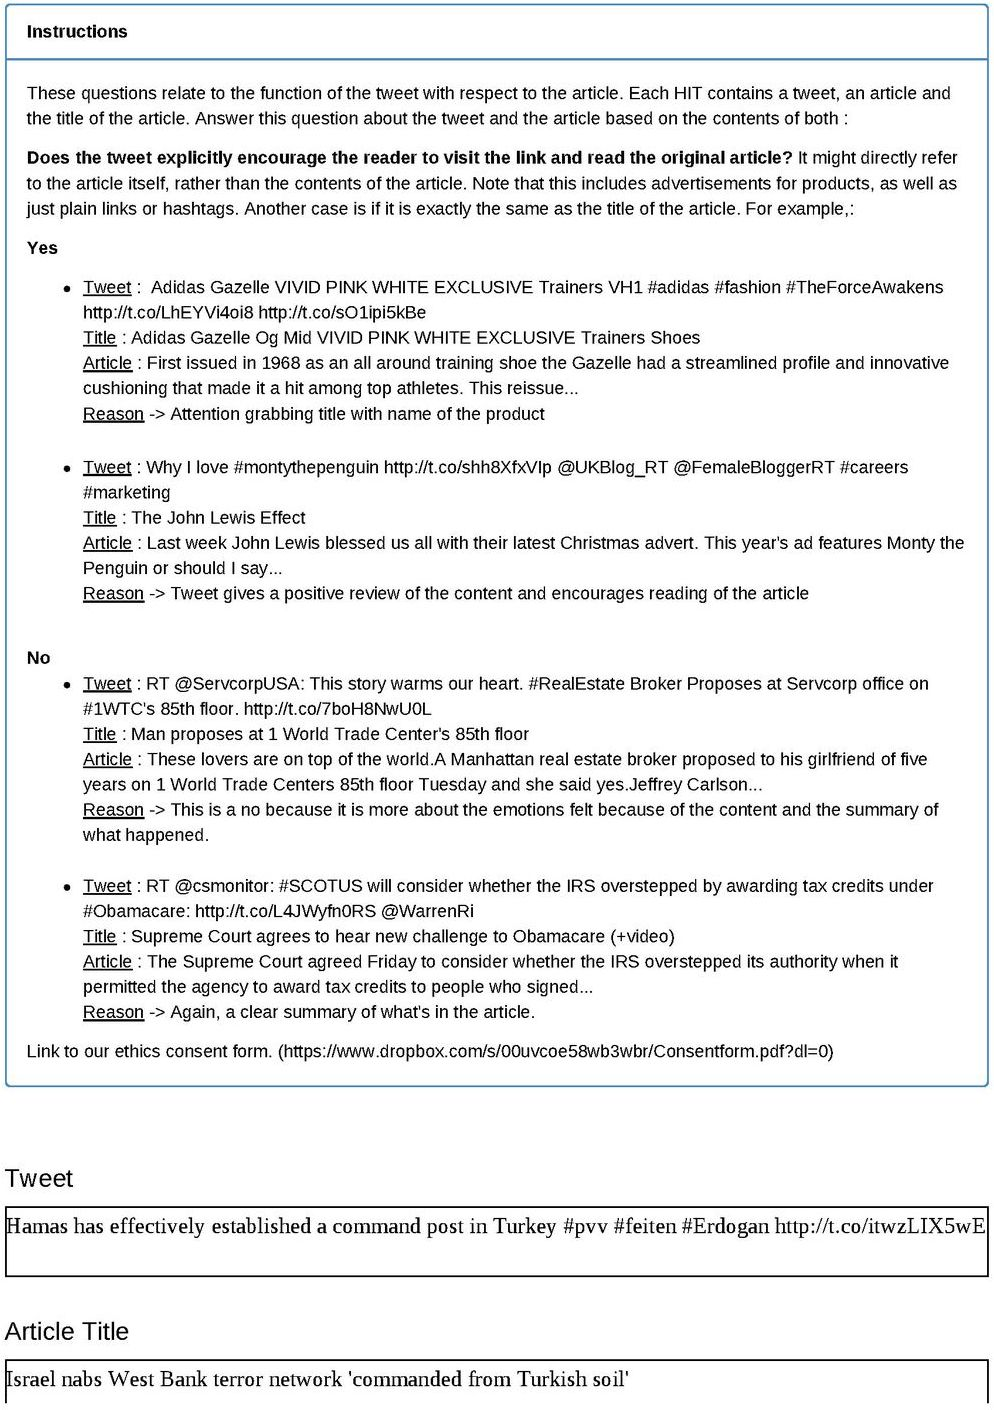
\includegraphics[width=\textwidth, height=21cm]{q11}}
  %\qquad 
  %\subfloat[][b]{q11} 
  \caption[User study question 1 example]{(a) The first question (Advertisement) posed for each sample asked to the users.}
  \label{fig:q1}
\end{figure}

\begin{figure}[!htbp]
  \ContinuedFloat 
  \centering 
  \subfloat{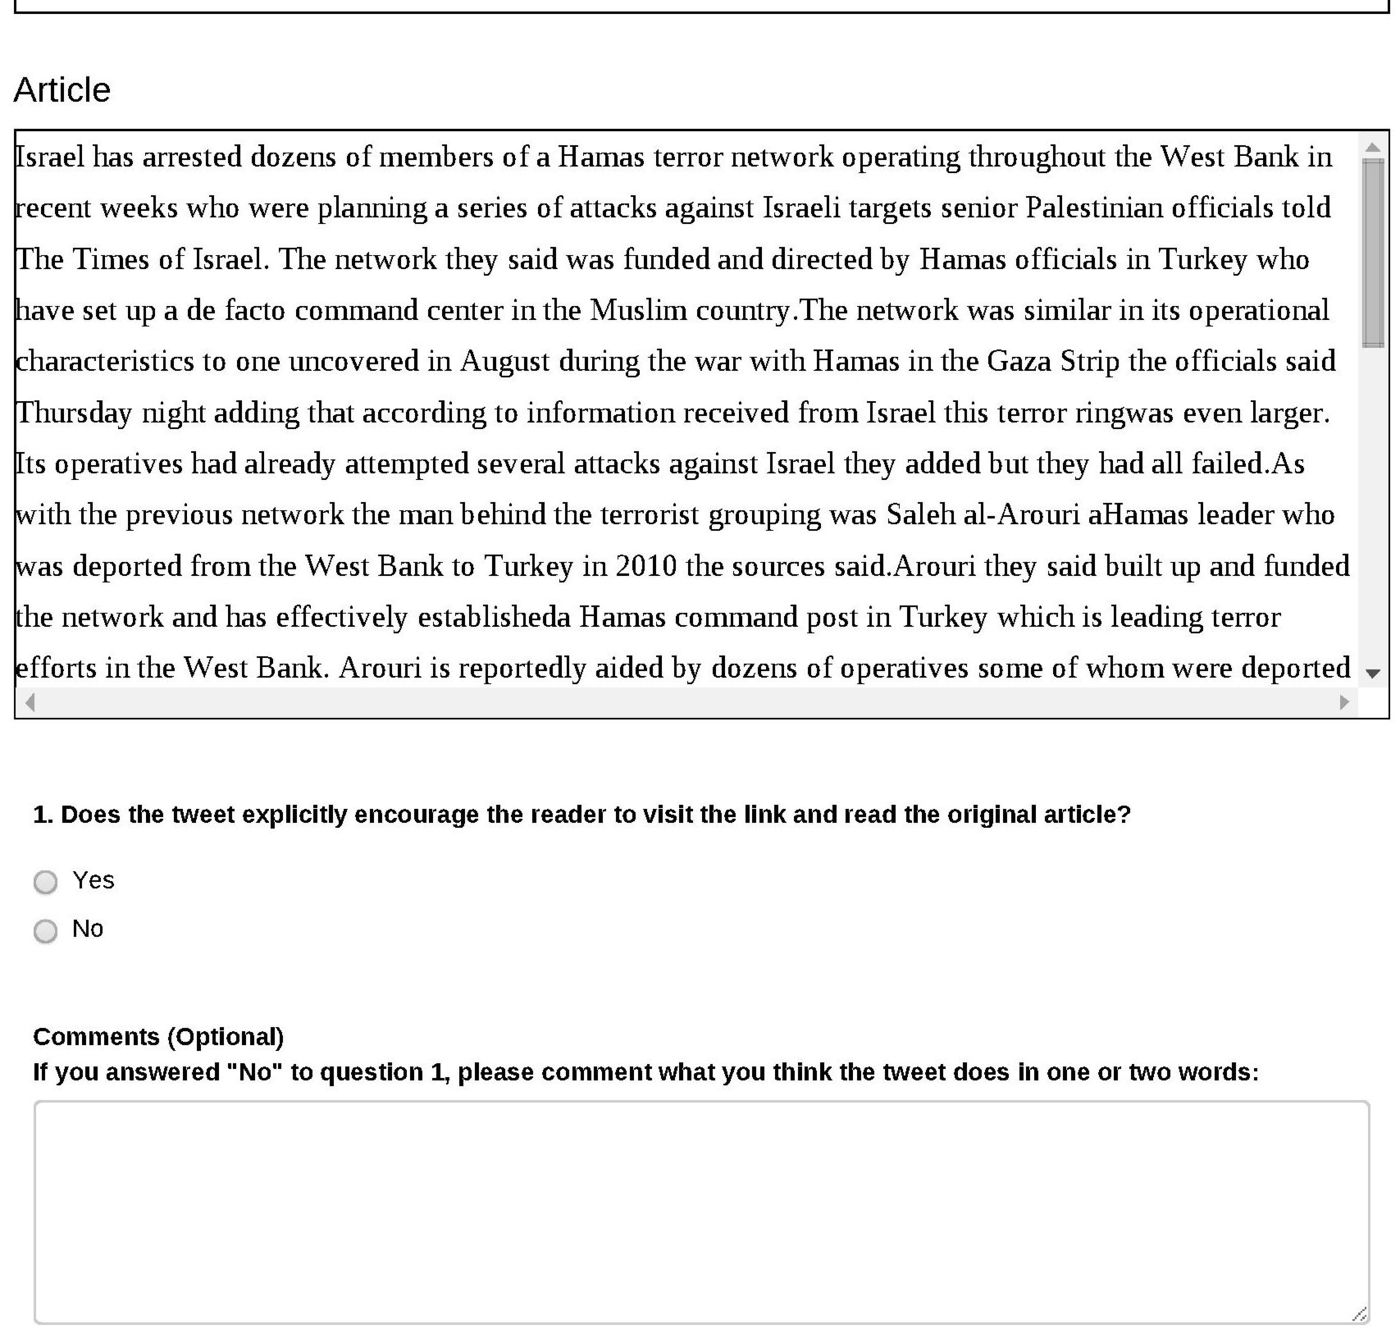
\includegraphics[width=\textwidth, height=13cm]{q12}}% 
  %\qquad 
  %\subfloat[][]{q12} 
  \caption[]{(b) The first question (Advertisement) posed for each sample asked to the users.}
  \label{fig:q12}
\end{figure} 

\begin{figure}[!htbp]
  \centering 
  \subfloat{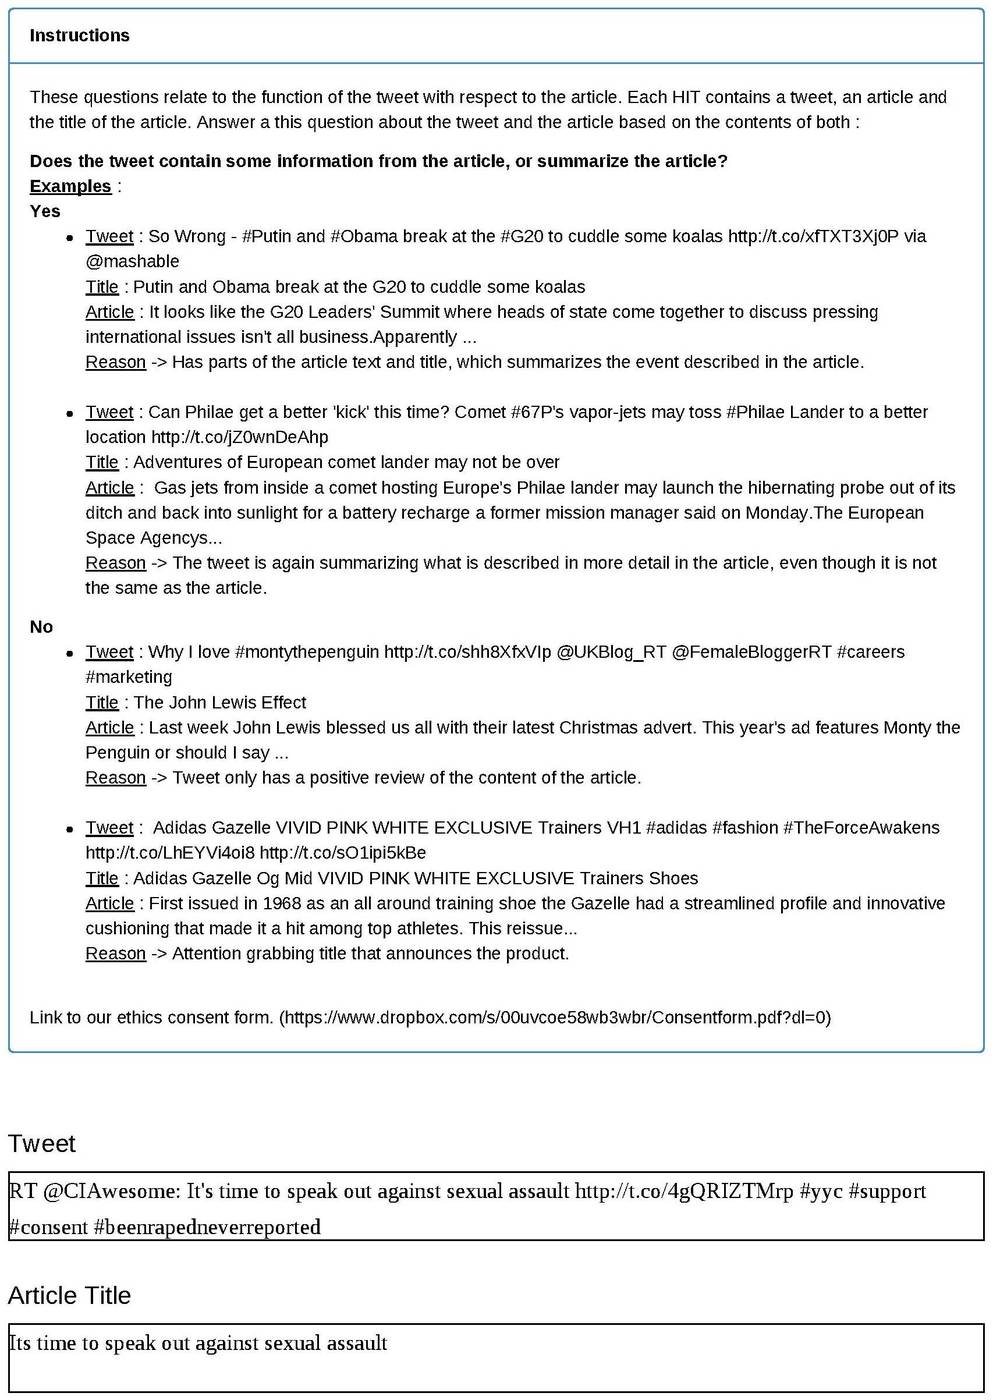
\includegraphics[width=\textwidth, height=21cm]{q21}}
  %\qquad 
  %\subfloat[][b]{q11} 
  \caption[User study question 2 example]{(a) The second question (Summary) asked for each sample.}
  \label{fig:q2}
\end{figure}

\begin{figure}[!htbp]
  \ContinuedFloat 
  \centering 
  \subfloat{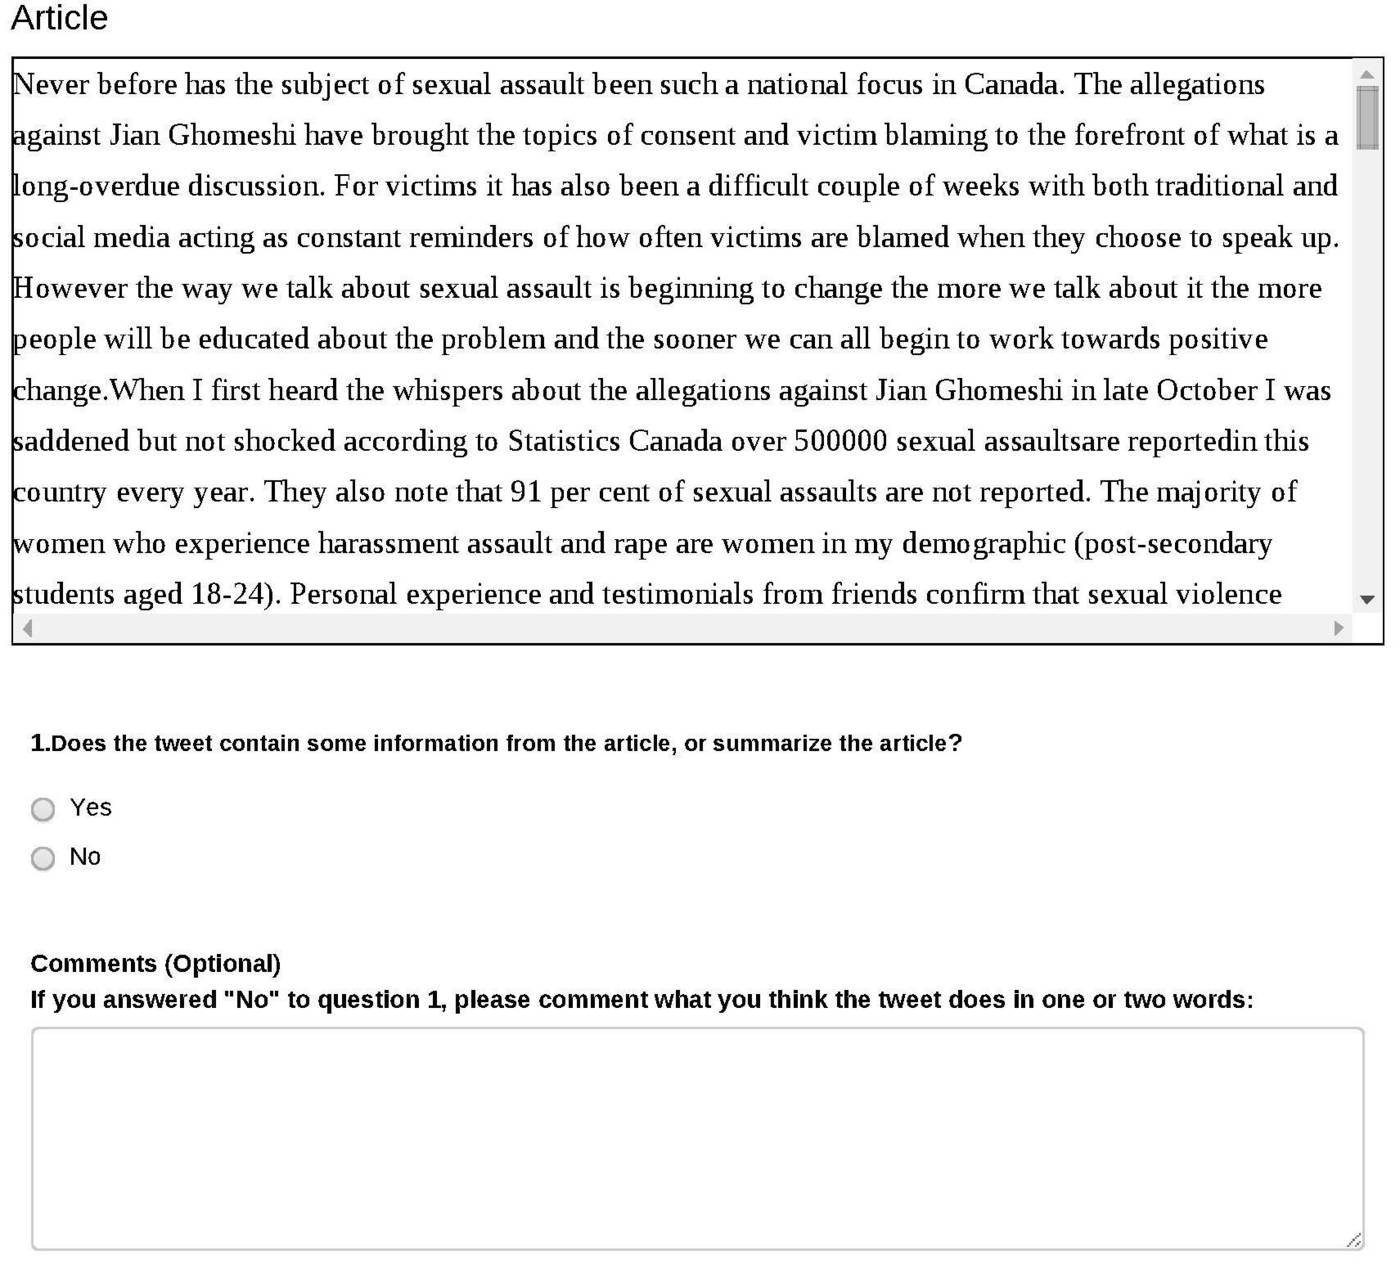
\includegraphics[width=\textwidth, height=13cm]{q22}}% 
  %\qquad 
  %\subfloat[][]{q12} 
  \caption[]{(b) The second question (Summary) asked for each sample.}
  \label{fig:q22}
\end{figure} 

\subsection{Qualification Details}

Mechanical Turk assigns qualifications to workers based on their skill level in answering questions and the percentage of accepted answers. Workers with superior skills and higher accuracy while answering HITs are given the qualification `Master' by Mechanical Turk, which was the qualification used for these pilot studies.

Three separate opinions from the workers were gathered for each tweet and article pair and the inter-annotator agreement was calculated using Fleiss' kappa measure  of agreement \citep{geertzen2012inter} between the raters. 

We found that the way to obtain the best quality results was to add an additional level of qualification over the default Master's qualification. The qualification test contained three tweet-article pairs from the dataset that had an obvious category for function of tweets. The test was conducted separately for the two questions asked. These tests were presented to the workers, and only workers with a 100\% score were allowed to work on the data. These tests ensured that the worker had a complete understanding of the task at hand. A separate pilot study with these qualifications and questions structure gave promising results, and the user study was then run on the entire dataset.

\subsection{Pilot Studies}
\label{sec:pilot}
Before finalizing the design of the study, we considered various different options, which will be discussed further in this section.

\paragraph{Attempts at tagging data} Our first attempt at tagging the dataset was made using the following scheme: a sample set of 100 articles were tagged by two people, based on the title, the article and the tweet. The tags used in the preliminary tagging were `evaluative', `descriptive', and `mixed'. `Evaluative' text is a more opinionated text, while `Descriptive' text is non-evaluative, containing, for example, a narration of an event or an explanation about a certain object or event. A `mixed' category was also added during tagging to accommodate some articles that could fall in either category. It was observed that this classification was rather subjective. \cite{liu2012survey} give a detailed analysis on classifying evaluative vs descriptive texts, which is called as subjectivity classification. They point out that it is a bad idea to classify on a sentence level in complex sentences, since a sentence and by extension a text might be factual as well as evaluative, which was the original problem while tagging. This tagging scheme did not yield much success in terms of gleaning information over the entire dataset.

\paragraph{Pilot studies for the user study} Four pilot studies were conducted sequentially on 100 different randomly selected tweet and article pairs each time, using each to improve the design for the next study. For these pilot studies, we tried various combinations of questions and qualifications, which are a type of grading system based on experience and ability for workers on Mechanical Turk.
 
\paragraph{A third possible function of tweets} Another possible question that was briefly mentioned in \secref{sec:qs} is whether the tweet expresses an opinion about something in the article. It could be a positive or a negative comment about the contents of the article, or an agreement or disagreement about the events, thoughts, and opinions expressed in the article. 

Example: ``This is a terrible analysis. \{url\}" or ``Listening to this album on repeat! \{url\}"

% However, it was dropped after a couple of pilot studies because of the difficulty in separating the emotion expressed towards the article as opposed to simply reiterating the emotion expressed in the article itself.

However, this question was dropped going forward with the studies because of the difficulty in distinguishing the difference between emotion towards the article vs emotion reiterated from the article itself.


\section{Results and Analysis for the User Study}

This section describes the analysis of results obtained from the user study.
% \begin{figure}[!htbp]
% \centering
% 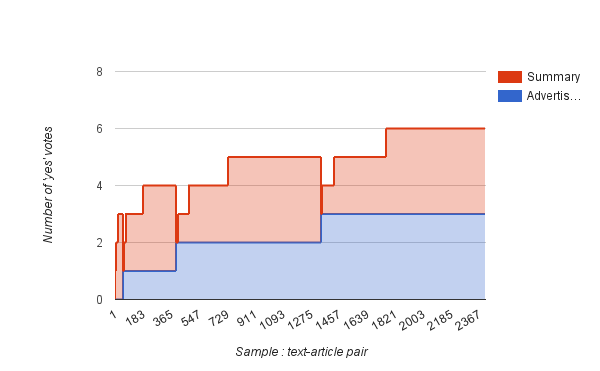
\includegraphics[width=0.9\textwidth, height=9cm]{results}
% \caption[Results from user study]{Visualization for tags from human evaluators}
% \label{fig:res}
% \end{figure}

% The results obtained from the final study are shown in \figref{fig:res}. The bottom line shows the number of 'yes' votes per article and tweet for the first question, whether the tweet was a promotion of the article. The red line on top of it signifies the number of 'yes' votes for the second question, whether the tweet was a summary of the article. 

The total number of `yes' votes for each of the questions are shown in \tabref{tab:yeses}. \tabref{tab:exq1no}, \tabref{tab:exq1yes}, \tabref{tab:exq2no} and \tabref{tab:exq2yes} all show examples where for one of each question, all three workers agreed on their answers to each of the two questions. The Fleiss' kappa for the first study, showing the indicativeness of the tweet was 0.147 and the kappa for the second study, showing the informativeness of the tweet, was 0.208.



We then analyzed the answers obtained from the study by correlating them with the overlap measures defined in \chapref{chap:analysis} with the help of the Mann Whitney U test \citep{mann1947test,wilcoxon1947probability}. The Mann Whitney U test considers two groups of ratings and then analyses them in terms of rankings to infer how they corroborate. Each of the following tables shows a result for the Mann Whitney U test for a study pertaining to one of the questions, and a corresponding analysis: unigram, bigram, or LCS matching percentages. \tabref{tab:unicorr1} and \tabref{tab:unicorr2} show the test results for unigram match percentages, \tabref{tab:bicorr1} and \tabref{tab:bicorr2} for bigram match percentages, and \tabref{tab:lcscorr1} and \tabref{tab:lcscorr2} for longest common subsequence match percentages. 

Mechanical Turk presents each question for each tweet-article pair to three different workers. Thus, every tweet-article pair has three different opinions for each question asked. We split all the tweet-article pairs from the data into two different groups. We form the groups for the Mann-Whitney U test using the above information. The first split considers zero `yes' votes in the answers as one group and three `yes' votes as another group. The second split considers zero or  one `yes' votes out of three in one group and two or three `yes' votes out of three in the other group. For each of these studies for each sample set configuration, the U statistic and the p value are shown. The final two columns in both tables show the mean of values in each of the groups used in the test. 
%The failure to reject the null hypothesis suggests that no definite distinction can be made between the degree of extraction for tweets that are advertisements for articles or summaries of articles.


\begin{table}[!t]
\centering
\begin{tabular}{|l|l|l|l|l|}
\hline
\textbf{Questions}     & \textbf{0 `yes' votes} & \textbf{1 `yes' vote} & \textbf{2 `yes' votes} & \textbf{3 `yes' votes}\\ \hline
Q1: Advertisement & 53    & 340    & 942     &  1068  \\ \hline
Q2: Summary       & 29     & 176    & 703     & 1495    \\ \hline
\end{tabular}
\caption{Analysis of user study results}
\label{tab:yeses}
\end{table}


\begin{table}[!t]
\centering
\begin{tabular}{|p{0.1\linewidth}|p{0.8\linewidth}|}
\hline
\textbf{Tweet} &   RT @WSJ: In \#CometLanding Philae probe bounced and settled in area that could hinder its research. http://t.co/6lfg3p9XG1 http://t.co/A6fi  \\ \hline
\textbf{Title} &   Rosetta Mission Probe Landed on Comet in Shadow of Cliff	                                                                                 \\ \hline
\textbf{Text}  &  The historic Philae comet probe hit its target but then unexpectedly bounced twice settling in the shadow of a cliff that could hinder its research new images sent back Thursday showed.Philae is designed to run a suite...                                                                                         \\ \hline
\end{tabular}
\captionof{table}{Example where all three workers said it was not an advertisement.}
\label{tab:exq1no}
\end{table}


\begin{table}[!t]
\centering
\begin{tabular}{|p{0.1\linewidth}|p{0.8\linewidth}|}
\hline
\textbf{Tweet} & \#GalaxyNote3 \#Lollipop - SamMobile has been teasing us with a number of unfinished builds for a few http://t.co/A0IKYsk4g3 \#Samsung \\ \hline
\textbf{Title} &   Samsung GALAXY Note 3's Android Lollipop Update Surfaces                                                                                 \\ \hline
\textbf{Text}  &  SamMobile has been teasing us with a number of unfinished builds for a few months now. This indicates...                                                                                         \\ \hline
\end{tabular}
\captionof{table}{Example where all three workers said the tweet was an advertisement for article.}
\label{tab:exq1yes}
\end{table}


\begin{table}[!t]
\centering
\begin{tabular}{|p{0.1\linewidth}|p{0.8\linewidth}|}
\hline
\textbf{Tweet} & "RT @jakbarali: So my partner Gillian Hnatiw and I had something to say about \#VAW \#LoriDouglas and \#Ghomeshi. http://t.co/6X2zMtCAM0 \\ \hline
\textbf{Title} & "Victim-blaming couched as legitimate judicial inquiry" \\ \hline
\textbf{Text}  & Ghomeshi himself broke the first wave of the story when he took to Facebook to decry the CBCs decision to terminate him... \\ \hline
\end{tabular}
\captionof{table}{Example where all three raters said the tweet was not a summary.}
\label{tab:exq2no}
\end{table}

\begin{table}[!t]
\centering
\begin{tabular}{|p{0.1\linewidth}|p{0.8\linewidth}|}
\hline
\textbf{Tweet} & RT @PopCulturPriest: Doing a story on California's lottery for @americmag I discovered \#JohnOliver's story had some troubling errors: http \\ \hline
\textbf{Title} & Blowing The Dismount: Last Week Tonight Fudges Its Lottery Story \\ \hline
\textbf{Text}  & Sunday night on the season finale of HBOs new news show Last Week Tonight anchor John Oliver spent half the show... \\ \hline
\end{tabular}
\captionof{table}{Example where all three raters agreed the tweet was a summary.}
\label{tab:exq2yes}
\end{table}

\begin{table}[!htbp]
\centering
\begin{tabular}{|p{0.29\textwidth}|p{0.1\textwidth}|p{0.1\textwidth}|p{0.09\textwidth}|p{0.09\textwidth}|p{0.09\textwidth}|p{0.09\textwidth}|}
\hline
\textbf{Groups considered}    & \textbf{U statistic} & \textbf{p value} & \textbf{Mean of values for Group 1} & \textbf{Number of samples in Group 1} & \textbf{Mean of values for Group 2} & \textbf{Number of samples in Group 2} \\ \hline
Group 1: 0 `yes' votes \newline Group 2: 3 `yes' votes &  28104  &  0.931413  &  27.44  & 53 & 28.21 &   1068  \\ \hline
Group 1: 0 or 1 `yes' votes \newline Group 2: 2 or 3 `yes' votes &   406355.5  & 0.365219 & 30.65  & 393 & 29.23 & 2010 \\ \hline
\end{tabular}
\caption{Mann Whitney U test results for the advertisement question(indicativeness): Unigram Match}
\label{tab:unicorr1}
\end{table}

\begin{table}[!htbp]
\centering
\begin{tabular}{|p{0.29\textwidth}|p{0.1\textwidth}|p{0.1\textwidth}|p{0.09\textwidth}|p{0.09\textwidth}|p{0.09\textwidth}|p{0.09\textwidth}|}
\hline
\textbf{Groups considered}    & \textbf{U statistic} & \textbf{p value} & \textbf{Mean of values for Group 1} & \textbf{Number of samples in Group 1} & \textbf{Mean of values for Group 2} & \textbf{Number of samples in Group 2}\\ \hline
Group 1: 0 `yes' votes \newline Group 2: 3 `yes' votes & 12211 & 0.000055  & 16.69 & 29 & 31.07 & 1495  \\ \hline
Group 1: 0 or 1 `yes' votes \newline Group 2: 2 or 3 `yes' votes & 193411 & 0.000791 & 25.08 & 205 & 29.87 & 2198 \\ \hline
\end{tabular}
\caption{Mann Whitney U test results for the summary question(informativeness): Unigram Match}
\label{tab:unicorr2}
\end{table}

\begin{table}[!htbp]
\centering
\begin{tabular}{|p{0.29\textwidth}|p{0.1\textwidth}|p{0.1\textwidth}|p{0.09\textwidth}|p{0.09\textwidth}|p{0.09\textwidth}|p{0.09\textwidth}|}
\hline
\textbf{Groups considered}    & \textbf{U statistic} & \textbf{p value} & \textbf{Mean of values for Group 1} & \textbf{Number of samples in Group 1} & \textbf{Mean of values for Group 2} & \textbf{Number of samples in Group 2}\\ \hline
Group 1: 0 `yes' votes \newline Group 2: 3 `yes' votes & 27871 & 0.851388 & 8.31 & 53 & 9.21 & 1068  \\ \hline
Group 1: 0 or 1 `yes' votes \newline Group 2: 2 or 3 `yes' votes& 406313 & 0.378553 & 12.19 & 393 & 10.29 & 2009 \\ \hline
\end{tabular}
\caption{Mann Whitney U test results for the advertisement question(indicativeness): Bigram Match}
\label{tab:bicorr1}
\end{table}

\begin{table}[!htbp]
\centering
\begin{tabular}{|p{0.29\textwidth}|p{0.1\textwidth}|p{0.1\textwidth}|p{0.09\textwidth}|p{0.09\textwidth}|p{0.09\textwidth}|p{0.09\textwidth}|}
\hline
\textbf{Groups considered}    & \textbf{U statistic} & \textbf{p value} & \textbf{Mean of values for Group 1} & \textbf{Number of samples in Group 1} & \textbf{Mean of values for Group 2} & \textbf{Number of samples in Group 2}\\ \hline
Group 1: 0 `yes' votes \newline Group 2: 3 `yes' votes & 15006 & 0.004541 & 3.88 & 29 & 11.46 & 1494  \\ \hline
Group 1: 0 or 1 `yes' votes \newline Group 2: 2 or 3 `yes' votes & 201755.5 & 0.013592 & 8.07 & 205 & 10.84 & 2197 \\ \hline
\end{tabular}
\caption{Mann Whitney U test results for the summary question(informativeness): Bigram Match}
\label{tab:bicorr2}
\end{table}



\begin{table}[!htbp]
\centering
\begin{tabular}{|p{0.29\textwidth}|p{0.1\textwidth}|p{0.1\textwidth}|p{0.09\textwidth}|p{0.09\textwidth}|p{0.09\textwidth}|p{0.09\textwidth}|}
\hline
\textbf{Groups considered}    & \textbf{U statistic} & \textbf{p value} & \textbf{Mean of values for Group 1} & \textbf{Number of samples in Group 1} & \textbf{Mean of values for Group 2} & \textbf{Number of samples in Group 2}\\ \hline
Group 1: 0 `yes' votes \newline Group 2: 3 `yes' votes &  26440.5  &  0.418424  &  42.16  & 53 &  44.24 &   1068  \\ \hline
Group 1: 0 or 1 `yes' votes \newline Group 2: 2 or 3 `yes' votes  &  392910     & 0.870236 &  44.66  & 393 & 44.69 & 2010 \\ \hline
\end{tabular}
\caption{Mann Whitney U test results for the advertisement question(indicativeness): Longest Common Subsequence}
\label{tab:lcscorr1}
\end{table}

\begin{table}[!htbp]
\centering
% \setlength\extrarowheight{5pt}
\begin{tabular}{|p{0.29\textwidth}|p{0.1\textwidth}|p{0.1\textwidth}|p{0.09\textwidth}|p{0.09\textwidth}|p{0.09\textwidth}|p{0.09\textwidth}|}
\hline
\textbf{Groups considered}    & \textbf{U statistic} & \textbf{p value} & \textbf{Mean of values for Group 1} & \textbf{Number of samples in Group 1} & \textbf{Mean of values for Group 2} & \textbf{Number of samples in Group 2}\\ \hline
Group 1: 0 `yes' votes \newline Group 2: 3 `yes' votes & 18466   & 0.171255 & 38.4 & 29 & 44.47  & 1495 \\ \hline
Group 1: 0 or 1 `yes' votes \newline Group 2: 2 or 3 `yes' votes & 217196.5      &  0.393999    & 43.16    & 205 & 44.83   &  2198\\ \hline
\end{tabular}
\caption{Mann Whitney U test results for the summary question(informativeness): Longest Common Subsequence}
\label{tab:lcscorr2}
\end{table}

The p-values for \tabref{tab:unicorr1}, \tabref{tab:bicorr1} and \tabref{tab:lcscorr1} show non-significant results for both sets of groups for the first question, the indicativesness of the tweet. The U statistic for each case is very high and the results show a $p>0.05$. We thus fail to reject the null hypothesis that the two sets were pulled from the same distribution. For all these cases, the means of the two groups are very close to the means for the respective analyis, and to each other. Mean for Unigram match is 29.53\%, mean for bigram match is 10.73\% and the mean for LCS match is 44.6\% as seen in \chapref{chap:analysis}. 
%The U statistic for each case is very high and the results show a $p>0.5$. We thus fail to reject the null hypothesis, that the two sets were pulled from the same distribution. The means of the LCS values, indicating the extractiveness of the tweet, are very close to each other. 

The p-values for unigram and bigram match for the second question, indicating the informativeness of the summary, shown in \tabref{tab:unicorr2} and \tabref{tab:bicorr2} are both significant, with $p<0.05$, especially so for the first arrangement of groups where group 1 is zero `yes' votes and group 2 is three `yes' votes. Based on the result of the p-values, we can conclude that these samples are drawn from different populations. If we look at the means of the values in each case, they are sufficiently different, with the mean of the first group being significantly smaller than the mean of the values in the second group. \tabref{tab:lcscorr2} also shows a slight difference in the means when zero vs three `yes' votes were considered as the sample set configuration. The U-statistic and p-value are both the least in this case for longest common subsequence results. However, no significant result can be drawn from this since the p-value is still quite high. It is possible that the non-significant result can be explained by the fact that the LCS is a lot more flexible for accommodating words from the overall article, and thus while the means of the two groups show difference in the right direction, the p-value is still too	 high to conclude anything significant. 

\subsection{Conclusions from the User Study}

The significant results from \tabref{tab:unicorr2} and \tabref{tab:bicorr2} represent evidence that tweets that are informative and tweets that are not informative have different levels of extractiveness from their source article. However, the evidence does not support the fact that whether a tweet is an advertisement interacts with the extractiveness of the tweet. Further studies would be required to come to a conclusion about this type of summary classification based on function, and how it interacts with extractiveness of the summary. The study shows a promising direction for further studies on the function of tweets. 

An important outcome of this chapter is the generation of a human-tagged dataset of tweet and article pairs, based on the indicativeness and informativeness of the tweets with respect to the article text. 

The question of whether a tweet summarizes the content of the article gave mostly positive answers, suggesting that according to the workers, if the tweet contained a link to article, it was an indicative summary in most cases. However, according to the extractiveness calculated earlier in \chapref{chap:analysis}, the tweets were not extracted from the articles to a large extent. With the results from the user study performed in this chapter, we can see that even when the tweet is used informatively, extractive methods have an upper bound that is still low, similar to what was obtained earlier. This reinforces the earlier conclusion of a need for a more sophisticated tool that summarizes the contents of the article for tweet generation.

% The question about whether a tweet summarizes the content of the article gave mostly postive answers, and the correlation with extractiveness shows that is the tweet is used informatively, then extractive methods give us a higher bound which still not helpful for generating tweets. This reinforces the earlier assumption that tweet generation must be done using a more sophisticated tool that summarizes the contents of the article.

%http://www.graphpad.com/guides/prism/6/statistics/index.htm?how_the_mann-whitney_test_works.htm

